%**************************
\chapter{Aritmética de las curvas elíptica}
\label{ch:Aritmética de las curvas elíptica}
%**************************

% conceptos han aparecido: extensión de cuerpo, característica, grupo

En el apartado~\ref{sec:Introducción} se introducen las curvas elípticas. Se explican las operaciones de grupo adicción y duplicacíon para los puntos de una curva elíptica, junto con su estructura fundamental y otras propiedades.

Las principales referencias usadas en este capítulo han sido~\cite{Washington:2008} y~\cite{Hankerson:2003}.

% TODO: seguir con la introducción de contenidos
% TODO: tengo que saber los teoremas que he referenciado como el teorema de Bezout o el teorema de Rienman-Roch.

\section{Introducción a las curvas elípticas}
\label{sec:Introducción}

% TODO: preguntarle a Pascual por la forma de citar (poner en el encabezado las principales referencias y despues para cosas puntuales usar \cite), pero no en cada definición o resultado no trivial.
\begin{definicion}
\label{def:curva elíptica}
	Una \emph{curva elíptica} $E$ se define por una una ecuación de la forma
	\begin{equation}
	\label{eq:Weierstrass general}
		E : y^2 + a_1 x y + a_3 y = x^3 + a_2 x^2 + a_4 x + a_6
	\end{equation}

	donde $a_1, a_2, a_3, a_4, a_6 \in K$ y $\Delta \neq 0$, donde $\Delta$ es el \emph{discriminante} de $E$ y se define como:

	\begin{align}
		\label{eq:discriminante}
		\begin{rcases}
		\Delta & = -d_2^2 d_8 - 8 d_4^3 - 27 d_6^2 + 9 d_2 d_4 d_6         \\
		d_2    & = a_1^2 + 4 a_ 2                                          \\
		d_4    & = 2 a_4 + 4 a_2                                           \\
		d_6    & = a_3^2 + 4 a_6                                           \\
		d_8    & = a_1^2 a_6 + 4 a_2 a_6 - a_1 a_3 a_4 + a_2 a_3^2 - a_4^2 \\
		\end{rcases}
	\end{align}

	Si $L$ es una extensión del cuerpo $K$, entonces el conjunto de puntos \emph{L-racionales} de $E$ es:
	$$
	E(L) = \{\infty\} \cup \{(x, y) \in L \times L: y^2 + a_1 x y + a_3 y = x^3 + a_2 x^2 + a_4 x + a_6 = 0\}
	$$
\end{definicion}

\begin{nota}[comentarios de la definición~\ref{def:curva elíptica}]\leavevmode
	\begin{itemize}
		\item La ecuación~\eqref{eq:Weierstrass general} se conoce como la \emph{ecuación de Weierstrass}.
		\item Diremos que $E$ \emph{está definida sobre} $K$ y lo notaremos $E/K$. A $K$ lo llamaremos \emph{cuerpo base}.
		\item La condición $\Delta \neq 0$ asegura que la curva elíptica es <<suave>>, esto es, no hay puntos en los que la curva tenga dos o mas rectas tangentes.
		% TODO: rellenar referencia a la forma proyectiva
		% TODO: cambiar si no se hace referencia al proyectivo (página 25 de washington)
		\item El punto $\infty$ lo llararemos \emph{punto del infinito}. Es el único punto en la linea del infinito que satisface la forma proyectiva de la ecuación de Weierstrass (véase~\ref{}).
		%\item A $\infty$ lo llamaremos \emph{punto del infinito}. En el apartado~\ref{} le daremos rigor y significado matemático a este nombre.
		%\item El punto $\infty$ es el único punto en la línea del infinito que satisface la forma proyectiva de la ecuación de Weierstrass (véase~\ref{}).
	\end{itemize}
\end{nota}

\begin{ejemplo}[curvas elípticas sobre $\mathbb{R}$]
	Consideramos las curvas elípticas:
	\begin{align*}
		E_1: y^2 & = x^3 - x \\
		E_2: y^2 & = x^3 + x
	\end{align*}
	definidas sobre el cuerpo $\mathbb{R}$ de los números reales. Los puntos $E_1(\mathbb{R})$ y $E_2(\mathbb{R})$ se han representado en la Figura~\ref{fig:curvas elípticas reales}.

	% TODO:hacer la gráfica bien (añadir label, etc, etc)
	\begin{figure}[h]
		\myfloatalign
		\subfloat[$E_1: y^2 = x^3 - x$]
		{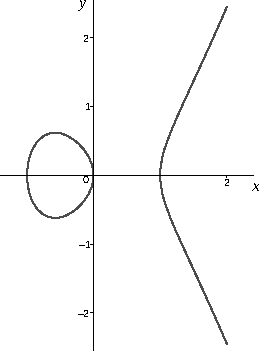
\includegraphics[width=.45\linewidth]{gfx/grafo_curva_eliptica_reales_1.pdf}} \quad
		\subfloat[$E_2: y^2 = x^3 + x$]
		{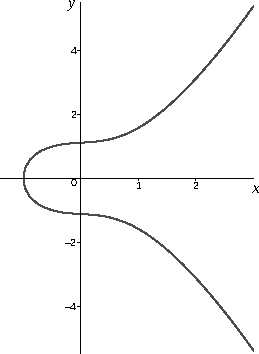
\includegraphics[width=.45\linewidth]{gfx/grafo_curva_eliptica_reales_2.pdf}}
		\caption{Curvas elípticas sobre $\mathbb{R}$}\label{fig:curvas elípticas reales}
	\end{figure}

	% \begin{figure}[h]
	% 	\centering
	% 	
\includegraphics[scale=1]{gfx/example_1}
	% 	\caption{Curvas elípticas sobre $\mathbb{R}$}\label{fig:curvas elípticas reales}
	% \end{figure}
\end{ejemplo}

\subsection{Ecuaciones de Weierstrass simplificadas}
\label{sub:Ecuaciones de Weierstrass simplificadas}

\begin{definicion}
	Dos curvas elípticas $E_1$ y $E_2$ definidas sobre $K$ y dadas por las ecuaciones de Weierstrass:
	\begin{align*}
		E_1 &: y^2 + a_1 x y + a_3 y = x^3 + a_2 x^2 + a_4 x + a_6 \\
		E_2 &: y^2 + a_1' x y + a_3' y = x^3 + a_2' x^2 + a_4' x + a_6'
	\end{align*}
	se dicen que son \emph{isomorfas sobre K} si existen $u, r, s, t \in K,\ u \neq 0$, tal que el cambio de variables lineal
	\begin{equation}\label{eq:cambio de variables admisible}
	(x, y) \mapsto (u^2 x + r, u^3 y + u^2 s x + y)
	\end{equation}
	transforma la ecuación $E_1$ en la ecuación $E_2$. La transformación~\eqref{eq:cambio de variables admisible} se llama un cambio de variables admisible.

	El cambio de variables~\eqref{eq:cambio de variables admisible} es el único que deja <<fijo>> el punto del infinito y preserva la forma de la ecuación de Weierstrass. No vamos a entrar en más detalle, pero puede consultar~\cite[prop. III.3.1b]{Silverman:2009} para más informácion.
\end{definicion}

% TODO: explicar porqué este cambio de variable referenciando a silverman

Una ecuación de Weierstrass
$$
E:  y^2 + a_1 x y + a_3 y = x^3 + a_2 x^2 + a_4 x + a_6
$$
puede simplificarse considerablemente aplicando cambios de variables admisibles. Usaremos las ecuaciones simplificadas en vez de la general en el resto del trabajo. Vamos a considerar por separado los casos en los que el cuerpo base tenga característica distinta de 2 y 3 o tenga característica 2 o 3.

\begin{enumerate}
	\item Si la característica de $K$ es distinta de $2$ y $3$, entonces el cambio de variables admisible
	$$
	(x, y) \mapsto \left(\frac{x - 3 a_1^2 - 12 a_2}{36}, \frac{y - 3 a_1 x}{216} - \frac{a_1^3 + 4 a_1 a_2 - 12 a_3}{240}\right)
	$$
	transforma $E$ en la curva
	\begin{equation*}\label{eq:ecuación Weierstrass}
		y^2 = x^3 + a x + b
	\end{equation*}
	donde $a, b \in K$. El discriminante de esta curva es $\Delta = -16(4a^3 + 27b^2)$.

	\item Si la característica de K es 2, hay dos casos que considerar. Si $a_1 \neq 0$, entonces el cambio de variables admisible
	$$
	(x, y) \mapsto \left(a_1^2 x + \frac{a_3}{a_1}, a_1^3 y + \frac{a_1^2 a_4 + a_3^2}{a_1^3} \right)
	$$
	transforma $E$ en la curva
	\begin{equation*}
		y^2 + xy = x^3 + a x^2 + b
	\end{equation*}
	% TODO: rellenar referencia
	donde $a, b \in K$. Tales curvas se llaman \emph{no supersingulares} (véase~\ref{}) y tienen discriminante $\Delta = b$. Si $a_1 = 0$, entonces el cambio de variables admisible
	$$
	(x, y) \mapsto (x + a_2, y)
	$$
	transforma $E$ en la curva
	\begin{equation*}
		y^2 + c y = x^3 + a x + b
	\end{equation*}
	% TODO: rellenar referencia
	donde $a, b, c \in K$. Tales curvas se llaman \emph{supersingulares} (véase~\ref{}) y tienen discriminante $\Delta = c^4$.

	\item Si la característica de $K$ es 4, entonces hay dos casos que considerar. Si $a_1^2 \neq -a_2$, entonces el cambio de variables admisible
	$$
	(x, y) \mapsto \left(x + \frac{d_4}{d_2}, y + a_1 x + a_1 \frac{d_4}{d_2} + a_3 \right)
	$$
	donde $d_2 = a_1^2 + a_2$ y $d_4 = a_4 - a_1 a_3$, transforma $E$ en la curva
	\begin{equation*}
		y^2 = x^3 + a x^2 + b
	\end{equation*}
	% TODO: rellenar referencia
	donde $a, b \in K$. Tales curvas se llaman \emph{no supersingulares} (véase~\ref{}) y tiene discriminante $\Delta = -a^3 b$. Si $a_1^2 = -a_2$, entonces el cambio de variables admisible
	$$
	(x, y) \mapsto (x, y + a_1 x + a_3)
	$$
	transforma $E$ en la curva
	\begin{equation*}
		y^2 = x^3 + a x^2 + b
	\end{equation*}
	% TODO: rellenar referencia
	donde $a, b \in K$. Tales curvas se llaman \emph{supersingulares} (véase~\ref{}) y tiene discriminante $\Delta = -a^3$.
\end{enumerate}
\begin{proof}
La demostración completa puede encontrarse en~\cite[sec. III.1]{Silverman:2009}. Se trata simplemente de completar cuadrados y realizar sustituciones, por ello aquí solo mostraremos la demostración de la primera simplificación.

En primer lugar, sumando en la ecuación de Weierstrass~\eqref{eq:Weierstrass general} en ambos lados por $(a_1 a_3 x)/2 + a_3^2/4 + (a_1^2 x^2)/4$, completamos el cuadrado:
$$
\left(y + \frac{a_1 x}{2} + \frac{a_3}{2}\right)^2 = x^3 + \left(a_2 + \frac{a_1^2}{4}\right)x^2 + \left(a_4 + \frac{a_1 a_3}{2}\right)x + \left(a_6 + \frac{a_3^2}{4}\right)
$$
Haciendo $y_1 = y + (a_1 x)/2 + a_3/2$, obtenemos
$$
y_1^2 = x^3 + a_2' x^2 + a_4' x + a_6'
$$
para algunas constantes $a_2', a_4', a_6' \in K$. Finalmente, sustituyendo $x_1 = x + a_2'/3$ resulta
$$
y_1^2 = x_1^3 + a x_1 + b
$$
para algunas constante $a, b \in K$. Para obtener el discriminante $\Delta$ basta sustiuir el valor de las constantes $a_4 = a,\ a_6 = b$ y $a_1 = a_3 = a_2 = 0$ en~\eqref{eq:discriminante}.
\end{proof}

\subsection{Ley de grupo}
\label{sub:Ley de grupo}

Sea $E$ una curva elíptica definida sobre un cuerpo $K$. Hay un \emph{método de la cuerda y la tangente} para sumar dos puntos en $E(K)$ y obtener un tercer punto en $E(K)$. Junto con esta operación aditiva, el conjunto de puntos $E(K)$ forma un gurpo abeliano con $\infty$ como elemento neutro.

La regla aditiva se explica fácilmente geométricamente. Sea $P$ y $Q$ dos puntos distintos de una curva elíptica $E$. Entonces la \emph{suma} $R$, de $P$ y $Q$ esta definido como sigue. Se dibuja una recta $L$ de $P$ a $Q$. Esta recta intersecta la curva elíptica en un tercer punto. Entonces $R$ es la reflexión de este punto sobre el eje-$x$. Esto se puede apreciar en la Figura~\ref{fig:ejemplo adicción}.

El \emph{doble} $R$, de $P$, se define como sigue. Se dibuja la línea tangente $L$ a la curva elíptica en $P$. Esta línea intersecta la curva elíptica en un segundo punto. Entonces $R$ es la reflexión de esto punto sobre el eje-$x$. Esto se puede apreciar en la Figura~\ref{fig:ejemplo duplicación}.

\begin{figure}[h]
  \myfloatalign
  \subfloat[Adicción: $P + Q = R$]{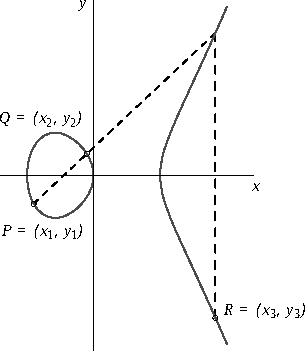
\includegraphics[width=.45\linewidth]{gfx/ejemplo_adiccion.pdf}\label{fig:ejemplo adicción}}
  \quad
  \subfloat[Duplicación: $P + P = P$]{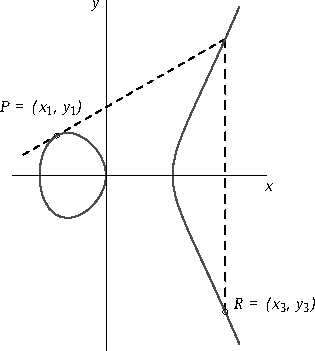
\includegraphics[width=.45\linewidth]{gfx/ejemplo_duplicacion.pdf}\label{fig:ejemplo duplicación}}
  \caption{Adicción y duplicación geométrica de puntos de una curva elíptica}\label{fig:Adicción y duplicación geométrica de puntos de una curva elíptica}
\end{figure}

El hecho de que $L \cap E$, contando multiplicidades, consiste en exactamente tres puntos (no necesariamente distintos) es un caso especial del teorema de Bézout~\cite[sec. I.7.8]{Hartshorne:1977}. Sin embargo, como vamos a dar fórmulas explícitas posteriormente en esta sección, no hay necesidad de usar un teorema general.

\begin{definicion}[ley de grupo]
\label{def:ley de grupo}
Sea $E$ una curva elíptica definida por la ecuación $y^2 = x^3 + a x + b$ sobre un cuerpo $K$ de característica distinta de 2 y 3. Definimos la operación binaria $+: E(K) \times E(K) \to E(K)$ como sigue:
\begin{enumerate}[label=\alph*)]
	\item $P + \infty = \infty + P = P,$ para todo $P \in E(K)$
	\item Si $P = (x, y) \in E(K)$, entonces $(x, y) + (x, -y) = \infty$. El punto $(x, -y)$ se denotará por $-P$ y se llamará el \emph{negativo} de P. Además, $- \infty = \infty$.
	\item Sea $P = (x_1, y_1) \in E(K)$ y $Q = (x_2, y_2) \in E(K)$, donde $P \neq \pm Q$. Entonces $P + Q = (x_3, y_3)$, donde
	$$
	x_3 = \left(\frac{y_2 - y_1}{x_2 - x_1}\right)^2 - x_1 - x_2, \quad
	y_3 = \left(\frac{y_2 - y_1}{x_2 - x_1}\right) (x_1 - x_3) - y_1
	$$
	\item Sea $P = (x_1, y_1) \in E(K)$, donde $P \neq \pm P$. Entonces $2 P = (x_3, y_3)$ donde:
	$$
	x_3 = \left(\frac{3 x_1^2 + a}{2 y_1}\right)^2 - 2 x_1, \quad
	y_3 = \left(\frac{3 x_1^2 + a}{2 y_1}\right) (x_1 - x_3) - y_1
	$$
\end{enumerate}
\end{definicion}
\begin{proof}
Tenemos que comprobar que $+$ es una operación binaria válida, esto es, que a cada par de elementos de $E(K) \times E(K)$ le corresponde un único elemento de $E(K)$. Como la casuística anterior es total y exclusiva, basta ver que $+$ es una operación cerrada. Los casos $a)$ y $b)$ son triviales. Veamos los otros dos casos con detalle.

\paragraph{Caso $c)$}
Supongamos $P = (x_1, y_1),\ Q = (x_2, y_2),\ P, Q \in E(K)$ con $P \neq \pm Q$. Consideramos la recta que los contiene:
$$
	L: y = m(x - x_1) + y_1,\ \text{donde}\ m = \frac{y_2 - y_1}{x_2 - x_1}
$$
Nótese que $x_2 \neq x_1$ ya que $P \neq \pm Q$. Para hallar la intersección de L con E sustituimos $y$:
$$
	(m(x - x_1) + y_1)^2 = x^3 + a x + b
$$
Podemos reescribir esto de la forma
\begin{equation}
\label{eq:cúbica}
	0 = x^3 - m^2 x^2 + b' x + c'
\end{equation}
para algunas constantes $b', c' \in K$. Así, las raíces de esta cúbica es justamente $L \cup E$.

Sabemos que las raíces de un polinomio están relacionadas con sus coeficientes. De hecho, para un polinomio cúbico mónico $x^3 + c_2 x^2 + c_1 x + c_0$ con raíces $r, s, t$ se tiene:
% -r s t  +  r s x  +  r t x  -  r x^2  +  s t x  -  s x^2  -  t x^2+x^3
\begin{align*}
	x^3 + &c_2 x^2 + c_1 x + c_0 = (x-r)(x-s)(x-t) \\
	&= x^3 - (r + s + t)x^2 + (r s + r t + s t)x - r s t
\end{align*}

En particular, $r + s + t = -c_2$. Como $P$ y $Q$ están en la intersección, $x_1$ y $x_2$ son dos raíces de~\eqref{eq:cúbica}, luego la tercera raíz $\alpha$ es $m^2 - x_1 - x_2$. Sustituyendo $\alpha$ en $L$ resulta $\beta = m(x_3 - x_1) + y_1$, luego $(\alpha, \beta) \in E(K)$. Entonces  $(\alpha, -\beta) = (x_3, y_3) \in E(K)$.

\paragraph{Caso $d)$}
Sea $P = (x_1, y_1)$, donde $P \neq -P$. Consideramos la recta tangente a $E$ en $P$
$$
	L: y = m(x - x_1) + y_1,\ \text{donde}\ m = \frac{3 x_1^2 + a}{2 y_1}
$$
Nótese que $y_1 \neq 0$ ya que si no estaríamos en el caso $b)$. Hallamos la intersección con E de forma análoga al caso $c)$ y obtenemos la cúbica:
$$
	0 = x^3 - m^2 x^2 + b' x + c'
$$
para algunas constantes $b', c' \in K$. Análogamente al caso $c)$, como $x_1$ es una raíz doble de la cúbica (derívese y evalúe en $x_1$) tenemos que la tercera raíz $\alpha$ es $m^2 - 2 x_1$. Sustituyendo $\alpha$ en $L$ resulta $\beta = m(x_3 - x_1) + y_1$, luego $(\alpha, \beta) \in E(K)$. Entonces  $(\alpha, -\beta) = (x_3, y_3) \in E(K)$.
\end{proof}

\begin{teorema}
	La suma~\ref{def:ley de grupo} de puntos en una curva elíptica $E$ sobre un cuerpo $K$ de característica distinta de 2 y 3 satisface la siguientes propiedades:
	\begin{itemize}
		\item \emph{Conmutatividad.} $P_1 + P_2 = P_2 + P_1,\ \forall P_1, P_2 \in E(K)$.
		\item \emph{Existencia de elemento neutro.} $P + \infty = P,\ \forall P \in E(K)$.
		\item \emph{Existencia de elemento opuesto.} $P + (-P) = \infty,\ \forall P \in E(K)$.
		\item \emph{Asociatividad.} $(P_1 + P_2) + P_3 = P_1 + (P_2 + P_3),\ \forall P_1, P_2, P_3 \in E(K)$.
	\end{itemize}
	En otras palabras, $(E(K), +, \infty)$ es un grupo abeliano.
\end{teorema}
\begin{proof}
La conmutatividad es trivial en los casos $a)$, $b)$ y $d)$. Para el caso $c)$ también es fácil ya que la recta que une $P_1$ y $P_2$ es la misma que la recta que une $P_2$ y $P_1$. La existencia de elemento neutro e inverso también es directo de la definición~\ref{def:ley de grupo}.

La asociatividad puede probarse utilizando las fórmulas caso por caso, pero supone un esfuerzo demasiado laborioso. En su lugar, puede abordarse de forma más sofisticada bien estudiando las líneas y sus intersecciones con la curva elíptica en el plano proyectivo~\cite[sec. 2.4]{Washington:2008} o bien usando teoremas más generales como el de Riemann-Roch~\cite[teo. III.3.4.e]{Silverman:2009}.
\end{proof}
